\section{Experiment}

This work presents the results of several experiments, dedicated to the $^{6,7}$H studies and one reference measurement of the same reaction mechanism, performed to control all the setup parameters and to test the reliability of the obtained results.
All the experiments were conducted in at the ACCULINNA-2 fragment separator \cite{Fomichev:2018}, recently constructed in the Flerov Laboratory of Nuclear Reaction of the Joint Institute for Nuclear Research. 
In this chapter, one briefly presents the main features of the ACCULINNA-2 facility and describes in more details the experimental setups, employed for the investigations of the isotopes of interest.

\subsection{ACCULINNA-2}

The idea of the ACCULINNA-2 in-flight separator is to provide, separate and transport the low-energy (from 10 to 40\,AMeV) RIBs of high intensity and purity. 
One should not, that it is not appropriate to compare its properties with those of such large facilities as FRS \cite{geissel:1992} and SuperFRS \cite{geissel:2003,winkler:2008} at FAIR, ARIS at FRIB \cite{gao:2015}, BigRIPS at RIKEN \cite{kubo:2003}, or others \cite{cuttone:2007,www:ganil,www:isolde}.
The scientific uniqueness of the ACCULINNA-2 facility is illustrated in Fig.\ \ref{fig:acculinna2_worldplace}.
One may see, that among all other in-flight separators, the chosen one is able to provide the light RIBs of the lowest possible energy, which is indispensable for certain experimental issues.
The technical approach of the facility allows one to provide a high energy and angular resolution of the secondary beams, which in conjunction with high efficiency for correlation measurements allows user to analyse multiple kinematic conditions of the projectile and the reaction products.  
That is why, selection of the studied reaction channel can be easily carried out, which, afterwards, leads to high quality of the spin-parity identification for the excitation spectra of the systems of interest.

%-------------------------------------------------------------------------------
\begin{figure}[t]
	\begin{center}
		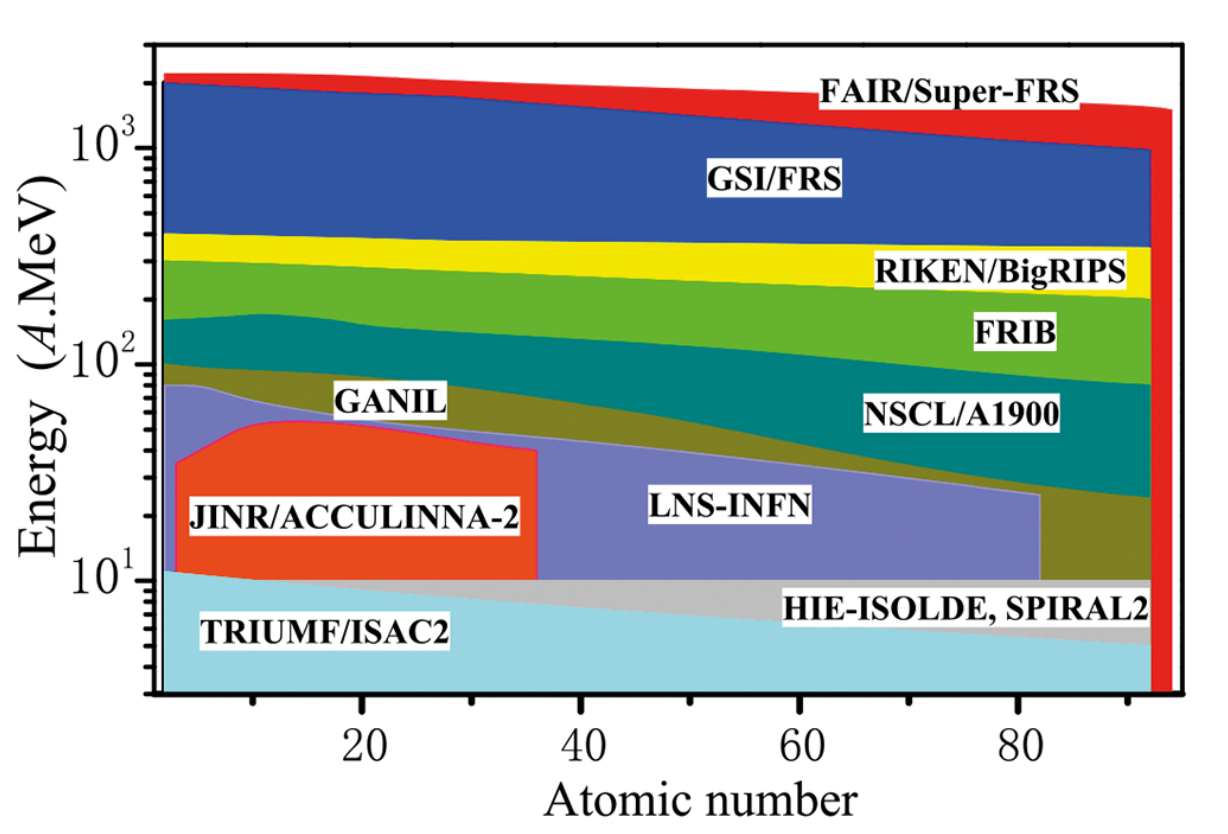
\includegraphics[width=0.7\textwidth]{figures/acculinna2_part.png}
	\end{center}
	%
	\caption{
		Landscape of the present-day facilities on the diagram where for radioactive beams, specified in terms of their atomic numbers, the available RIB energy ranges are shown.}
	%
	\label{fig:acculinna2_worldplace}
\end{figure}
%-------------------------------------------------------------------------------

The ACCULINNA-2 facility is coupled to the U400-M cyclotron, which provides high intensity primary beams of $^{7}$Li, $^{11}$B, $^{13}$C, $^{15}$N and $^{18}$O of energies  between 30 and 50\,AMeV.
Of course, the fragment separator can be configured in a mode to form the mentioned stable beams and deliver them into the reaction chamber.  
The ACCULINNA-2 facility is 36 meters long achromatic separator consisting of two 45-degree dipole magnets, 14 quadrupoles, eight multipoles (three octupoles and five sextupoles) and four steering magnets, see Fig.\ \ref{fig:acculinna2_scheme}.
The high intensity primary beams are delivered by the U-400M cyclotron to the rotating production target module installed in the first intermediate focal plane F1 to produce radioactive ion beams in fragmentation reactions via the in-flight method.

The production target module, integrates a vacuum chamber with a water cooled beryllium target mounted on rotating magnetic liquid feed through and a set of water-cooled diaphragms. 
The target module is designed to work with heating power up to 2\,kW. 
Radioactive nuclei leaving the production target are captured by a short-focusing quadrupole triplet Q1–Q3 and are transported through the magnetic dipoles D1–D2 and magnetic quadrupoles Q4–Q14 up to the final focal plane F5. 
Magnetic multipoles with corresponding sextupole and octupole components are used for correction of second- and third- order aberrations occurring otherwise in the F2 and F3 planes (see in Fig.\ \ref{fig:acculinna2_scheme}). 

The purification of the reaction fragments is achieved by a separation method based on magnetic-rigidity analysis and energy-loss in a degrader material. 
The D1 dipole magnet filters fragments by their magnetic rigidity $B$ , providing dispersion at the focal plane F2. 
The relation between the magnetic rigidity of the first bending magnet and the $A/Z$ number is given by $B=p/q$. 
Further purification is achieved by separation of the fragments by their energy losses in the wedge-shaped degrader. 
The second dipole D2 compensates the dispersion occurring in the focal plane F2 and collects the fragments at the achromatic focal plane F3. 
Identification of the reaction products is performed by the measurement of the Time of Flight (TOF) and energy
loss ($E$) of the fragments.
Both of them are measured by two scintillation detectors installed in the the F3 and F5 focal planes with 12.3-meter base. 
Each scintillator is coupled with four Hamamatsu R7600-200 photomultiplier tubes (PMT). 
With these devices one can reach the time resolution of 100\,ps, which determines the accuracy of determining of the beam kinetic energy.
The selection made for the thicknesses of the production target and wedge-shaped degrader in accord with the position determination made for the momentum slits standing in focal planes F2–F5 have direct influence on the yield and purity of the required RIB.
This is typically sufficient for the production of quite pure RIBs of light, neutron-rich exotic nuclei. Proton-rich RIBs need additional purification from a large amount of contamination. 
The reason of that is the fragmentation mechanism leads to the low-energy tails of obtained in the energy spectra of the very well-produced undesirable less proton-rich nuclei. 
Adding the velocity separation to the magnetic-rigidity analysis one can drastically reduce the effect of this contamination. 
For this purpose a radio-frequency (RF) kicker is installed in on the beam-line between the F3 and F4 focal planes (see in Fig.\ \ref{fig:acculinna2_scheme}). 

The secondary beam tracking is realized by pair of multi-wire proportional chambers (MWPC), placed at the distances of 28 and 81\,cm upstream of the experimental target plane, located in the reaction chamber.
The MWPCs are filled with CF$_{4}$ and CH$_{4}$ gas mixture with a ratio 9 to 1 and atmospheric presure.
Each detector consists of two layers, 32 wires each, installed with interval of 1.25\,mm. 
This allowed to determine the RIB interaction points in the target plane with a 1.8\,mm  precision.
Also, this beam-tracking installation determined the inclination angles of individual RIB projectiles to the ion optical axis with an accuracy of $\approx 0.15 $\,degrees.


%-------------------------------------------------------------------------------
\begin{figure}[t]
	\begin{center}
		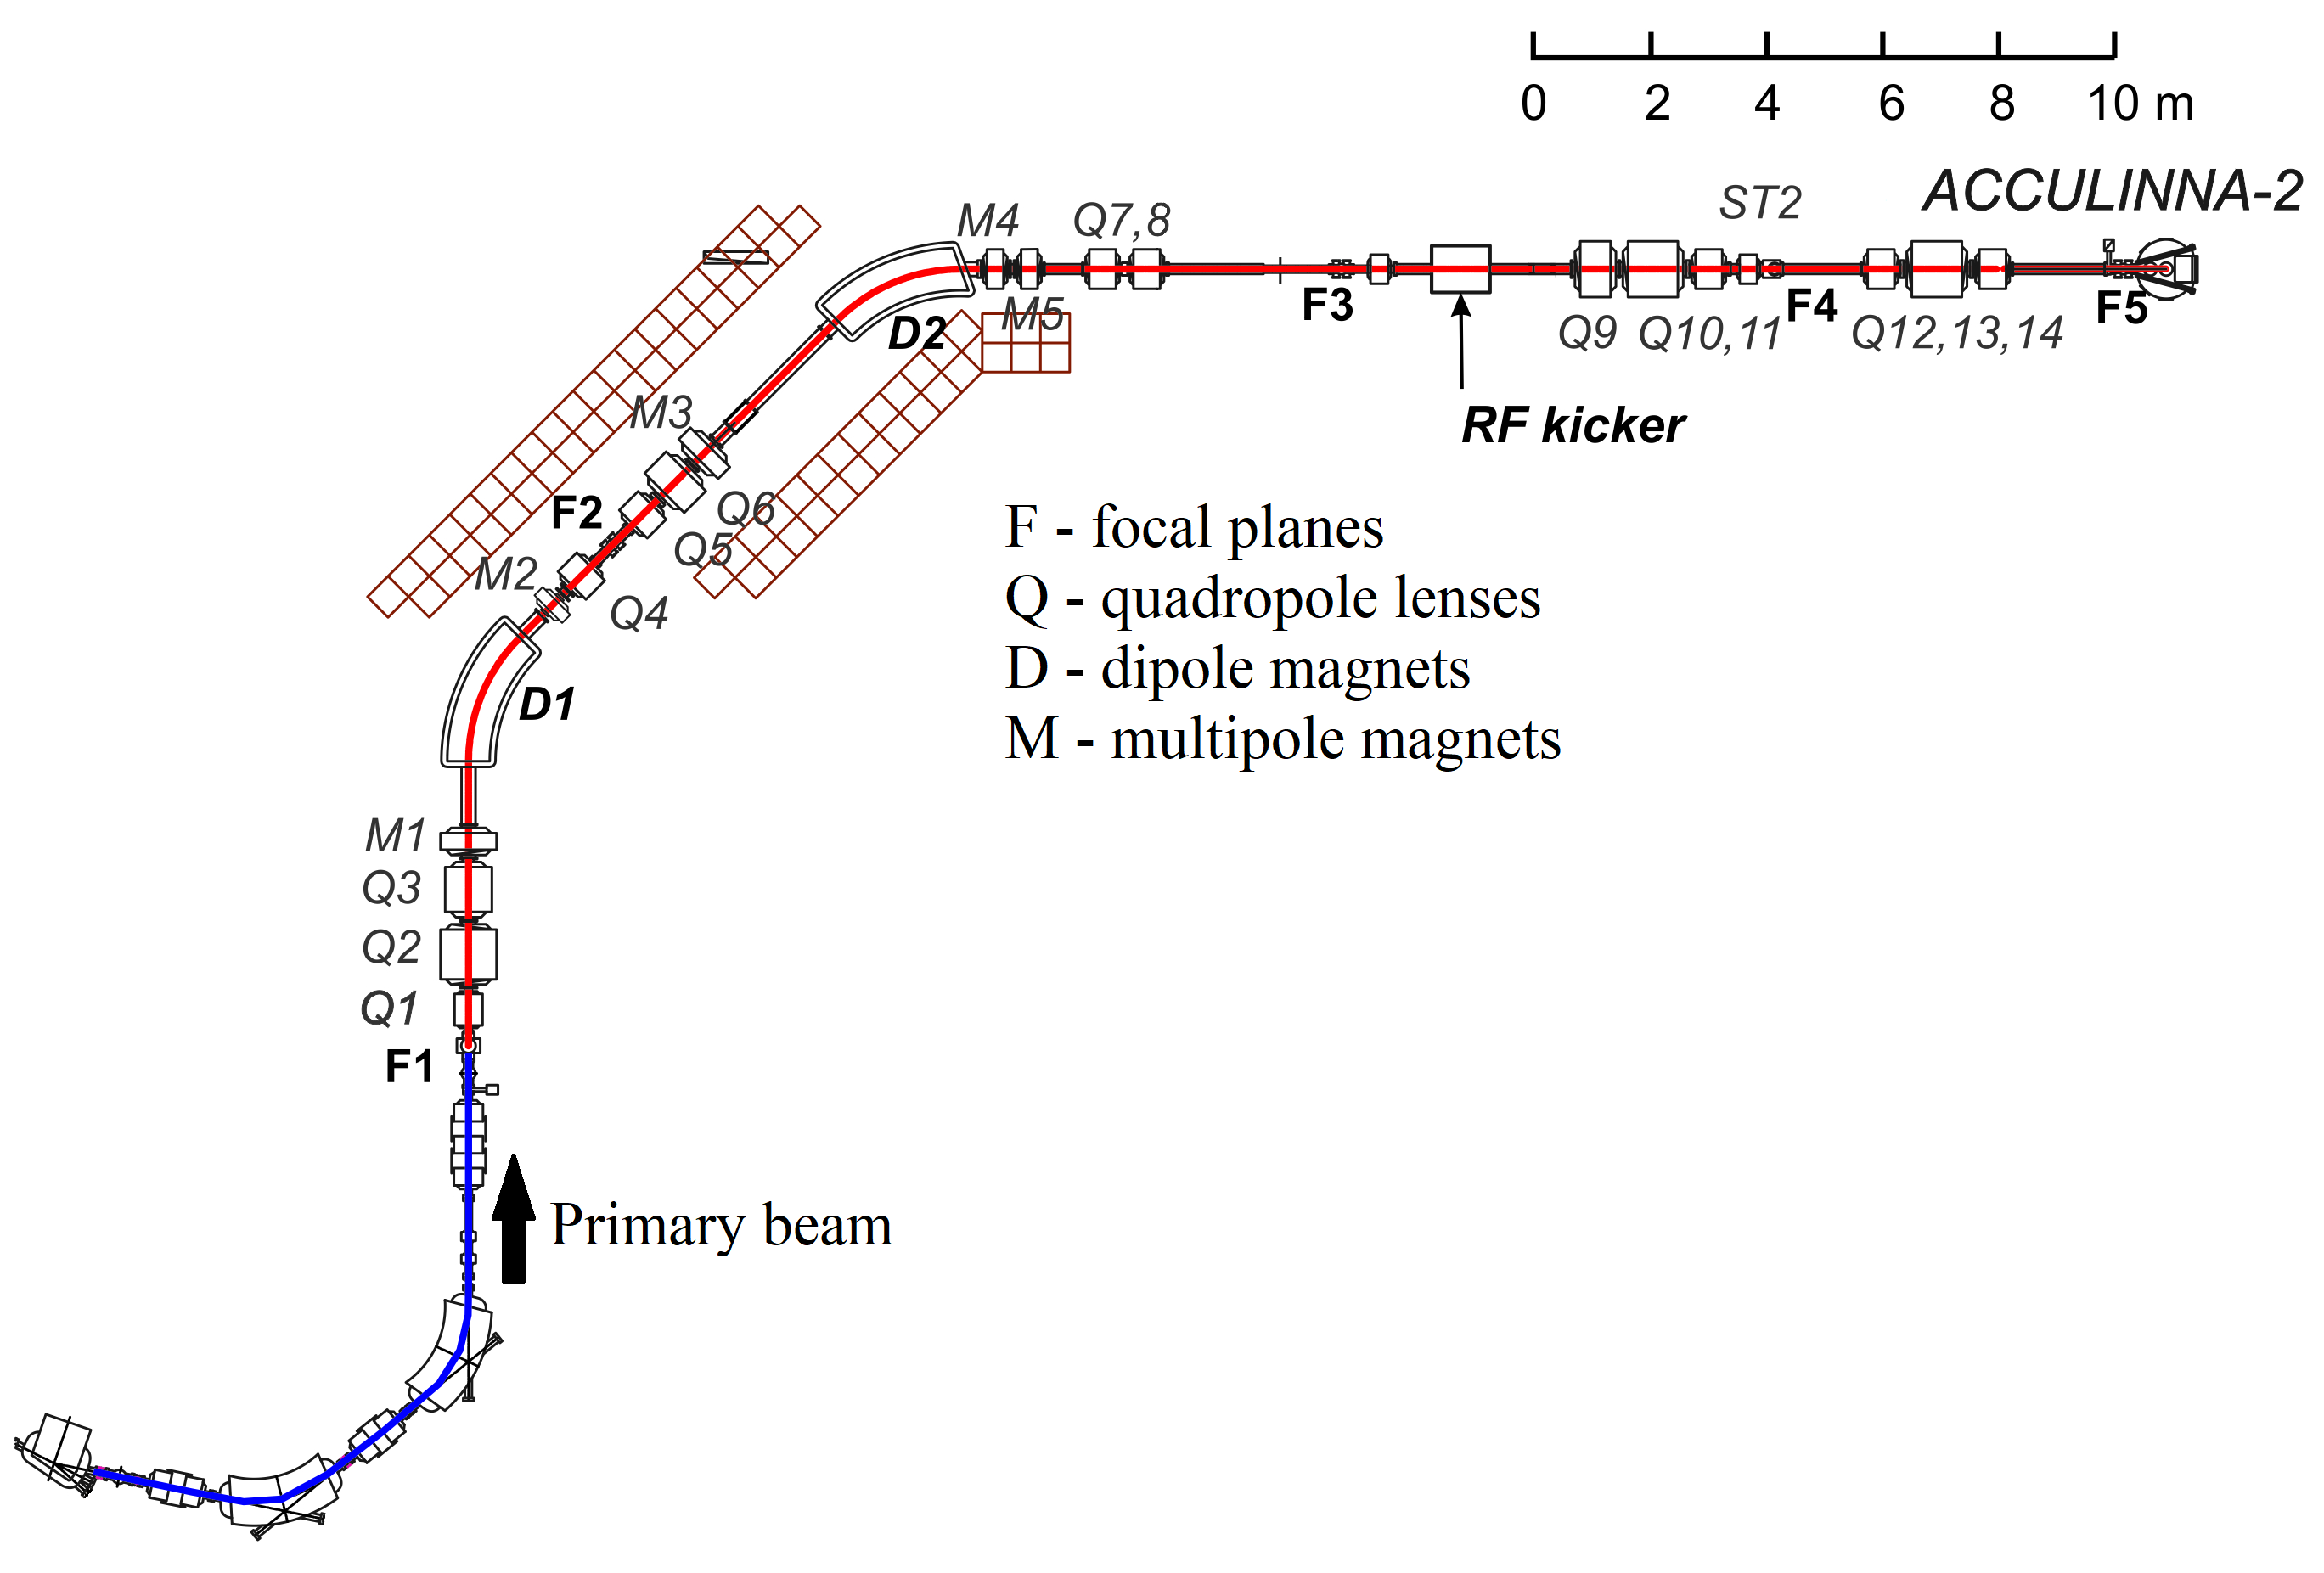
\includegraphics[width=1\textwidth]{figures/acculinna2.png}
	\end{center}
	%
	\caption{Lay-out of the fragment-separator ACCULINNA-2. F1 – the object plane; F2 – the intermediate dispersion plane; F3, F4 – the achromatic focal planes; F5 – the final focal plane.}
	%
	\label{fig:acculinna2_scheme}
\end{figure}
%-------------------------------------------------------------------------------

\subsection{Experimental setup}


